\section{Goal Conditioned Reinforcement Learning}

In Part 1, we will be running goal-conditioned $Q$-learning on two problems:
\begin{enumerate}
\item a toy problem where we flip bits in a bit vector to match it to the current goal vector
\item move the end effector of a simulated robotic arm to the desired goal position
\end{enumerate}

Applying hindsight relabeling to a goal-conditioned reinforcement learning setting is one of the most promising and commonly-used ways to improve sample efficiency and exploration challenges of RL!

\textbf{Setup:} Please navigate to \texttt{src/submission/goal\_conditioned\_rl} and follow the instructions in the \texttt{README.md}.

\textbf{Part 1 Code Overview:} The code consists of several files to enable $Q$-learning. All code
for Part 1 is located in the directory \texttt{src/submission/goal\_conditioned\_rl}. You are expected to write
the code in the following files: \texttt{run\_episode.py}, \texttt{trainer.py}. A brief description for the
codebase is provided here:

\begin{enumerate}
    \item \texttt{trainer.py}: The main training loop. Alternates between collecting transitions
using $Q$-value networks and training the networks on collected transitions.
\item \texttt{run\_episode.py}: Collects an episode using the current $Q$-value network, and returns
the transitions, collected reward and whether the agent was successful during the
episode.
\item \texttt{replay\_buffer.py}: Buffer for storing the transitions collected in the environment.
\item  \texttt{q\_network.py}: Creates a feedforward neural network with one hidden layer. This
neural net represents our $Q$-network.
\item  \texttt{bit\_flip\_env.py}: The source code for the bit flipping environment, which is set up
to follow the gym API with an \texttt{\_\_init\_\_}, \texttt{reset} and \texttt{step} functions.
\item \texttt{sawyer\_action\_discretize.py}: Wraps the SawyerReachXYEnv from multiworld environment and converts the continuous action space into a discrete action space with
a simplified 2D observation space.
\item \texttt{main.py}: Main file to configure the experiment.
\end{enumerate}

\textbf{Environments:}

You will be running RL methods on two environments:

\textbf{Environment 1: Bit Flipping Environment}
In the bit-flipping environment,
the state is a binary vector with
length $n$. The goal is to reach a
known goal vector, which is also
a binary vector with length $n$. At
each step, we can flip a single bit
in the vector (changing a 0 to 1 or
a 1 to 0). This environment can
very easily be solved without reinforcement learning, but we will
use the DQN algorithm to understand how adding hindsight relabelling  (HER) can improve performance. An example of this environment is shown in Table \ref{fig:bitflip}.


The bit flipping environment is an example of an environment with sparse rewards. At
each step, we receive a reward of -1 when the goal and state vector do not match and
a reward of 0 when they do. With a larger vector size, we receive fewer non-negative
rewards.

\begin{table}[h]
\centering
\begin{tabular}{ccccc}
\toprule
\textbf{Timestep} & \textbf{Current State} & \textbf{Action} & \textbf{Reward} & \textbf{Next State} \\
\midrule
1 & [1,0,0,0,1,1] & 0 & -1 & [0,0,0,0,1,1] \\
2 & [0,0,0,0,1,1] & 5 & -1 & [0,0,0,0,1,0] \\
3 & [0,0,0,0,1,0] & 3 & 0 & [0,0,0,1,1,0] \\
\bottomrule
\end{tabular}
\caption{Illustration of an example bit flipping environment with $n = 6$. The initial state of the environment is [1,0,0,0,1,1] and the goal is to reach the state [0,0,0,1,1,0].}
\label{fig:bitflip}
\end{table}

\textbf{Environment 2: 2D Sawyer Arm (Figure \ref{fig:sawyer})}

\begin{figure}[h]
\centering
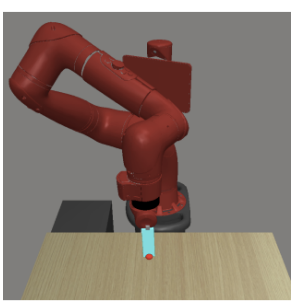
\includegraphics[width=0.3\textwidth]{figures/sawyer.png}
\caption{Illustration of an example Sawyer environment.}
\label{fig:sawyer}
\end{figure}

The Sawyer Arm (see Figure \ref{fig:sawyer}) is a multi-jointed robotic arm for grasping 
and reaching (\href{https://robots.ieee.org/robots/sawyer/}{see more details here}). The arm operates
in a 2D space, and the goal is to move the robot to a set of coordinates. The sawyer reach is an example of a dense reward environment,
where the reward is given by negative Euclidean distance between the
robot arm and the goal state. The end-effector (EE) is constrained to
a 2-dimensional rectangle parallel to a table. The action controls EE
position. The state is the XY position of the EE and the goal is an XY
position of the EE.

\begin{enumerate}[(a)]
    \item \points{1a} \textbf{Implementing Goal Conditioned Reinforcement Learning}

We start this problem with a goal-conditioned implementation of
DQN. The $Q$-function takes in the concatenated state and goal as input. You can think of the goal-conditioned implementation as an extended Markov decision process (MDP), where your state space contains both the original state and the goal. We will use this goal-conditioned $Q$-network to
collect episodic data in \texttt{run\_episode.py}.

For this part of the assignment, complete \texttt{run\_episode.py} and run the following command:
\begin{lstlisting}[language=bash]
    python -m goal_conditioned_rl.main --env bit_flip --num_bits=6 --num_epochs=250 --her_type no_hindsight
\end{lstlisting}

The evaluation metrics should be available in tensorboard events logged in \texttt{logs/} by default. \textbf{Verify} the \texttt{eval\_metrics}, that is \texttt{total\_reward} should be above $-40.0$ and success rate
should be $1.0$. This plot illustrates the performance without using HER.

\begin{center}
    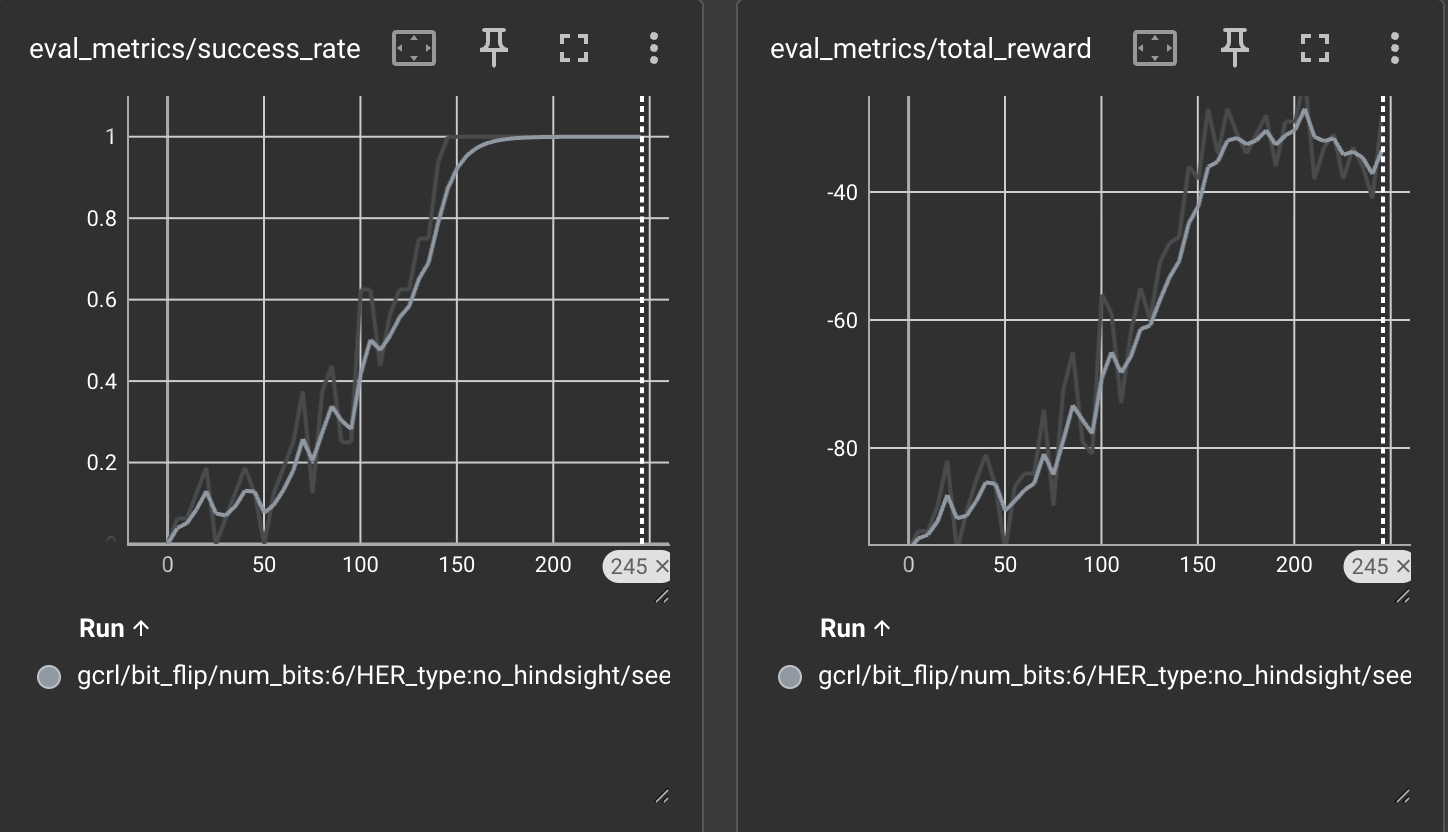
\includegraphics[width=0.5\textwidth]{figures/1a-expect}
\end{center}

\begin{enumerate}[label=(\roman*)]
    \item  For simplicity, we will only consider the \textit{greedy} action with respect to $Q$-network.
Pass this action to \texttt{env.step}.
\item The \texttt{env.step} function returns \texttt{next\_state}, \texttt{reward}, \texttt{done}, \texttt{info}, where \texttt{info} is a
dictionary containing the a boolean under the key '\texttt{successful\_this\_state}', indicating whether the state was successful or not. Use this value to update succeeded,
such that \texttt{run\_episode} returns \texttt{True} if the \textit{policy was successful at any step of the episode}.
To understand more about \texttt{env.step}, read the documentation for the function in
\texttt{bit\_flip\_env.py}.
\item Ensure that floating point numpy arrays use \texttt{np.float32}. You may need to recast
some of the arrays to ensure that.
\end{enumerate}
    \item \points{1b} \textbf{Adding HER to Bit Flipping}

With HER, the model is trained on the actual (state, goal, reward) tuples along with (state,
goal, reward) tuples where the goal has been relabeled after the fact. The goals are relabeled to the state that was \textit{actually reached} and the rewards should be relabeled correspondingly. In other words, we pretend that the state we reached was our goal all along. HER
gives us more examples of actions that lead to positive rewards, effectively doubling our
experience (since we use the original episode as well as the relabeled one). The reward
function for relabeled goals is the same as the environment reward function; for the bit
flipping environment, the reward is $-1$ if the state and goal vector do not match and 0 if
they do match.

There are three different variations of HER: \texttt{final}, \texttt{random}, and \texttt{future}. Suppose the data collected in an episode consists of the following (state, goal, reward) tuples: $\{(s_t, g, r_t)\}_{t=0}^T$, where $t$ indicates each time step in the episode. Given a (state, goal, reward) tuple $(s_i, g_i, r_i)$ each variation of HER relabels the goal $g_i$ differently:

\begin{itemize}
    \item \texttt{final}: The final state of the episode is used as the goal.
    
    \item \texttt{random}: A random state in the episode is used as the goal.
    
    \item \texttt{future}: A random future state of the episode is used as the goal. Specifically, if you want to relabel the goal in the tuple $(s_i, g_i, r_i)$, only states $s_j$ with $j > i$ can be used.
\end{itemize}

Implementation Notes:

\begin{itemize}
    \item Always use \texttt{copy()} when assigning an existing numpy array to a new variable. NumPy does not create a new copy by default.
    
    \item When choosing a new goal for relabelling, choose the state corresponding to \texttt{next\_state} from the experience.
\end{itemize}

More details of these three implementations are in the comments of \texttt{trainer.py}. Implement the three variations of HER in the function \texttt{update\_replay\_buffer} in \texttt{trainer.py}. You \textbf{do not} need to submit a plot for this.



    \input{02-goal-conditioned-rl/03-analyze-bit-flip}
    \input{02-goal-conditioned-rl/04-analyze-baseline}
    \input{02-goal-conditioned-rl/05-analyze-sawyer-search}
    \item \points{1f} \textbf{Bit Flipping Environment Logs}

For this question, please run our zip script to collect all your logs for the bit flipping environment with different number of bits and HER types. To verifiy
if you submission is looking find, review and compare your folder structure with the one below:

\dirtree{%
.1 submission.
.2 goal\_conditioned\_rl.
.3 *.
.3 logs.
.4 gcrl.
.5 bit\_flip.
.6 num\_bits/6.
.7 HER\_type/final.
.8 seed/42 (or another number if you choose to use a different seed).
.9 YOUR\_TF\_FILE.
.7 HER\_type/no\_hindsight.
.8 seed/42 (or another number if you choose to use a different seed).
.9 YOUR\_TF\_FILE.
.6 num\_bits/15.
.7 Same as num\_bits/6 but with runs for final/future/no\_hindsight/random.
.6 num\_bits/25.
.7 Same as num\_bits/6 but with runs for final/no\_hindsight.
.6 sawyer\_reach.
.7 Same as num\_bits/6 but with runs for final/no\_hindsight.
}
\end{enumerate}
